\subsection{Initial temperature for melting}

When looking at the simulation in Ovito, we found that the melting point seems to be around an initial temperature of 600 K. 

Not melted 600 K

Melted 650 K


Tell if the system is solid? When is it melting?


\subsection{Real melting temperature}

The system starts in a very ordered state, so the potential energy is very low. In the first time step the atoms have moved away from this high symmetric low potential state and the potential energy increases very much. Because the total energy has to be conserved, the kinetic energy decreases a lot to compensated. The drop in kinetic energy gives a drop in temperature because of the relating between them (see Equation \ref.). Figure \ref{fig:temperature} shows the development of the temperature with time. The temperature is approximately half the initial temperature in equilibrium. 

\begin{figure}[H]
\center
\includegraphics[width=0.8\linewidth]{../figures/temp_development}\caption{This is a  plot of the ratio between the initial temperature and the temperature calculated from the kinetic energy (see Equation \ref.) to show how it decreases to an equilibrium which is approximately half the initial temperature.}\label{fig:temperature}
\end{figure}


What temp is it really melting at?


\subsection{Diffusion constant}

Something is wrong - high diffusion constants at low T and the other way around?

\begin{figure}[H]
\center
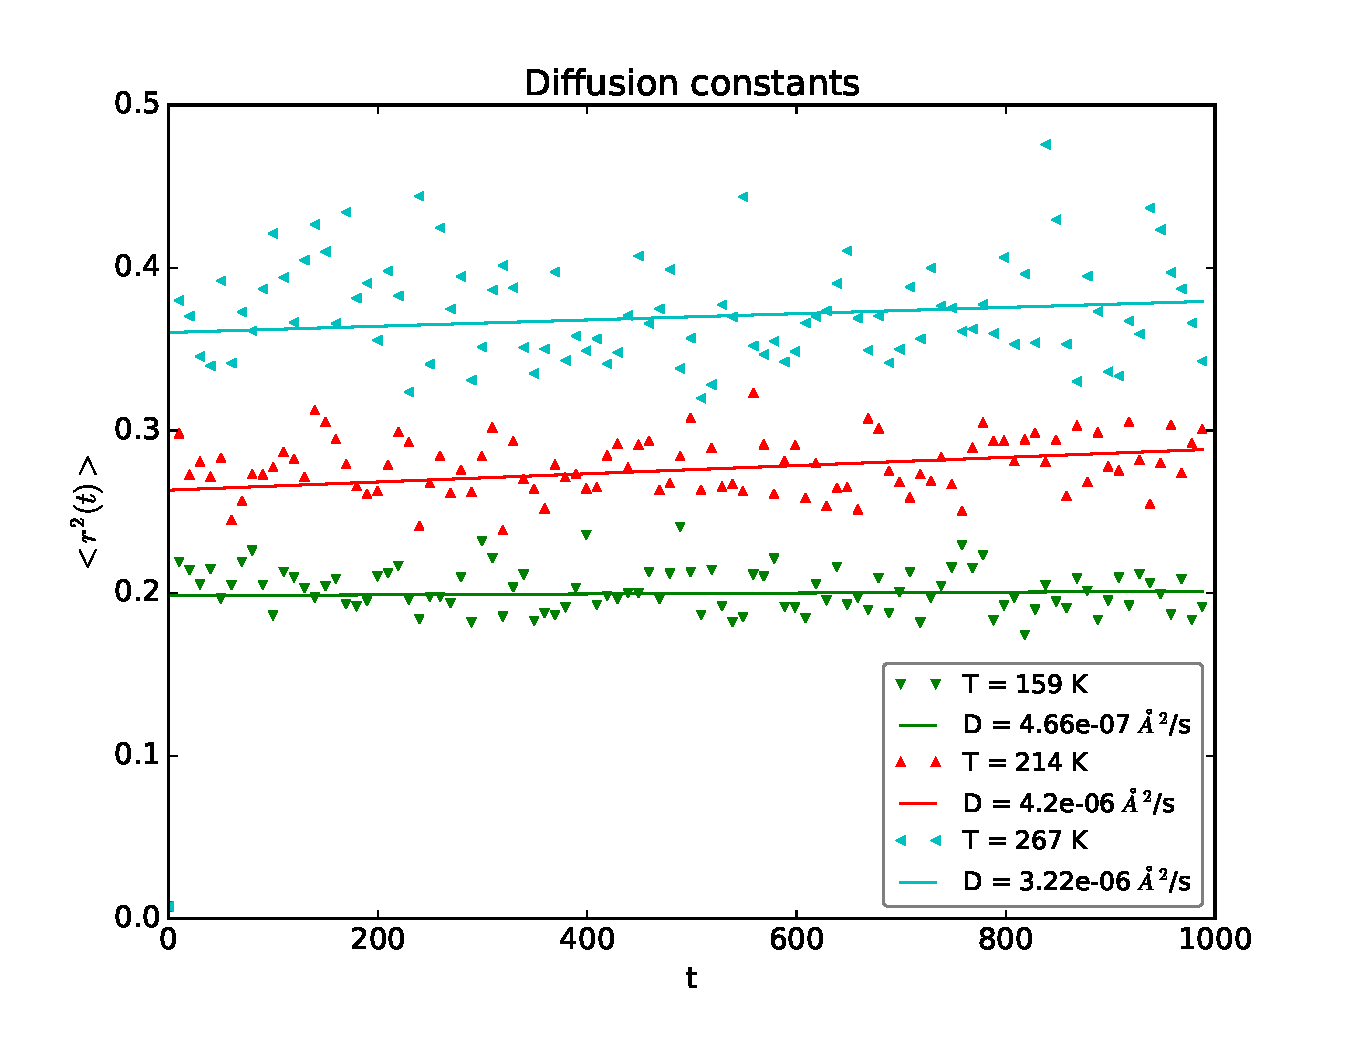
\includegraphics[width=0.8\linewidth]{../figures/diffusion_constants_low}\caption{This is a plot of Einstein relation, the diffusion constant is extraced from the slope of the linear regression.}\label{fig:diffusion_low}
\end{figure}

\begin{figure}[H]
\center
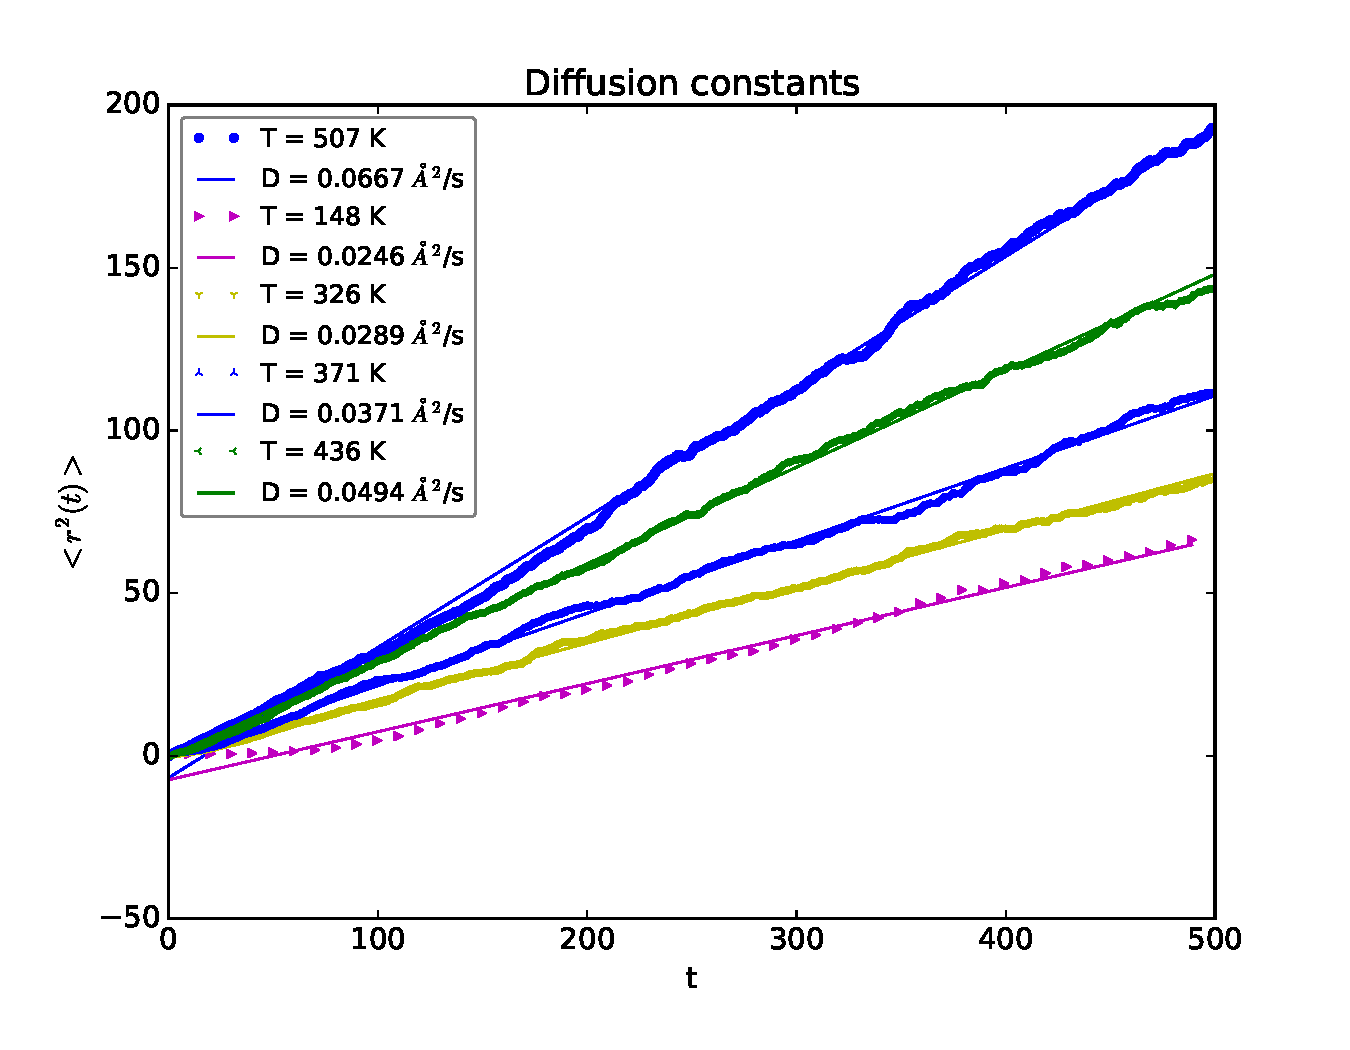
\includegraphics[width=0.8\linewidth]{../figures/diffusion_constants_high}\caption{This is a plot of Einstein relation, the diffusion constant is extraced from the slope of the linear regression.}\label{fig:diffusion_high}
\end{figure}

\begin{figure}[H]
\center
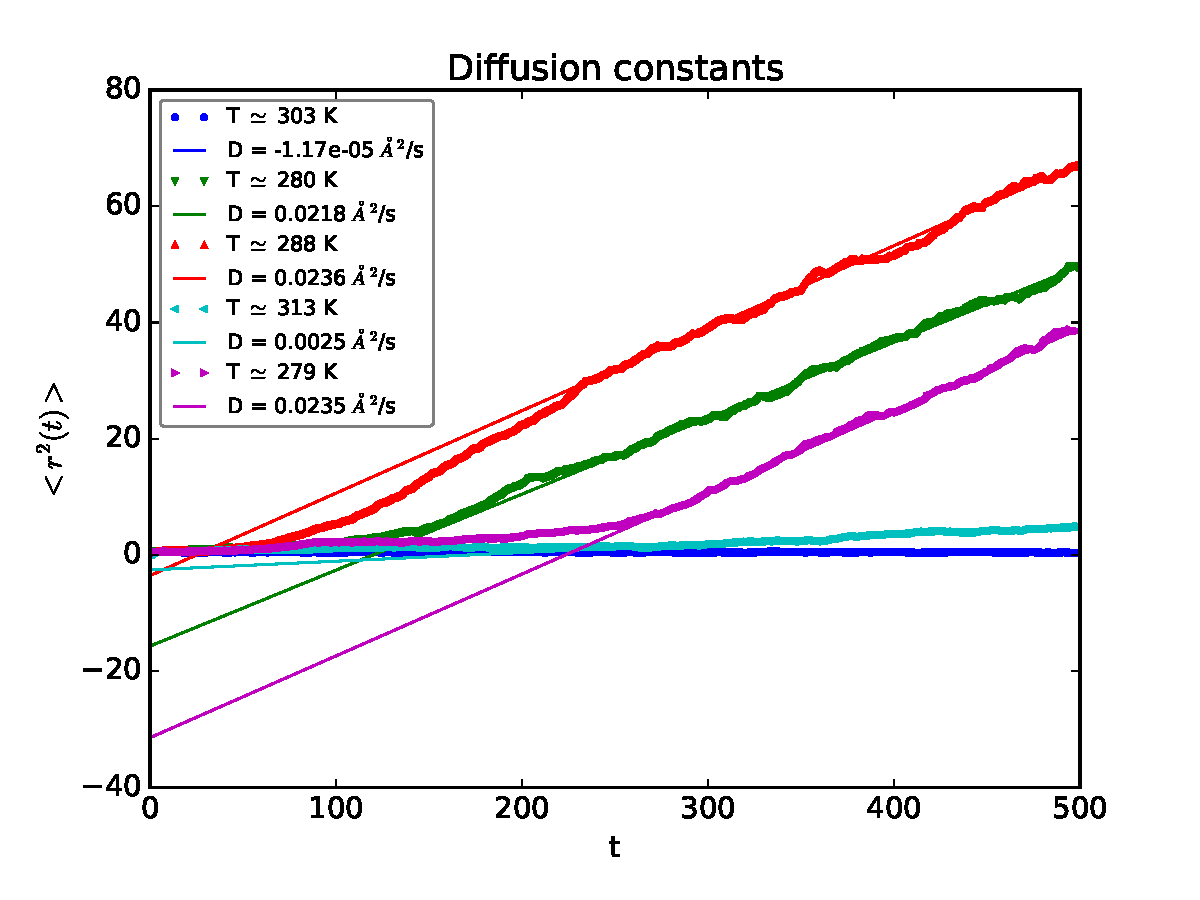
\includegraphics[width=0.8\linewidth]{../figures/diffusion_constants}\caption{This is a plot of Einstein relation, the diffusion constant is extraced from the slope of the linear regression. The temperature is near the phase transition between solid and liquid/gas.}\label{fig:diffusion_near_Tc}
\end{figure}


Should we only find the linear regression where the data looks linear?

\begin{figure}[H]
\center
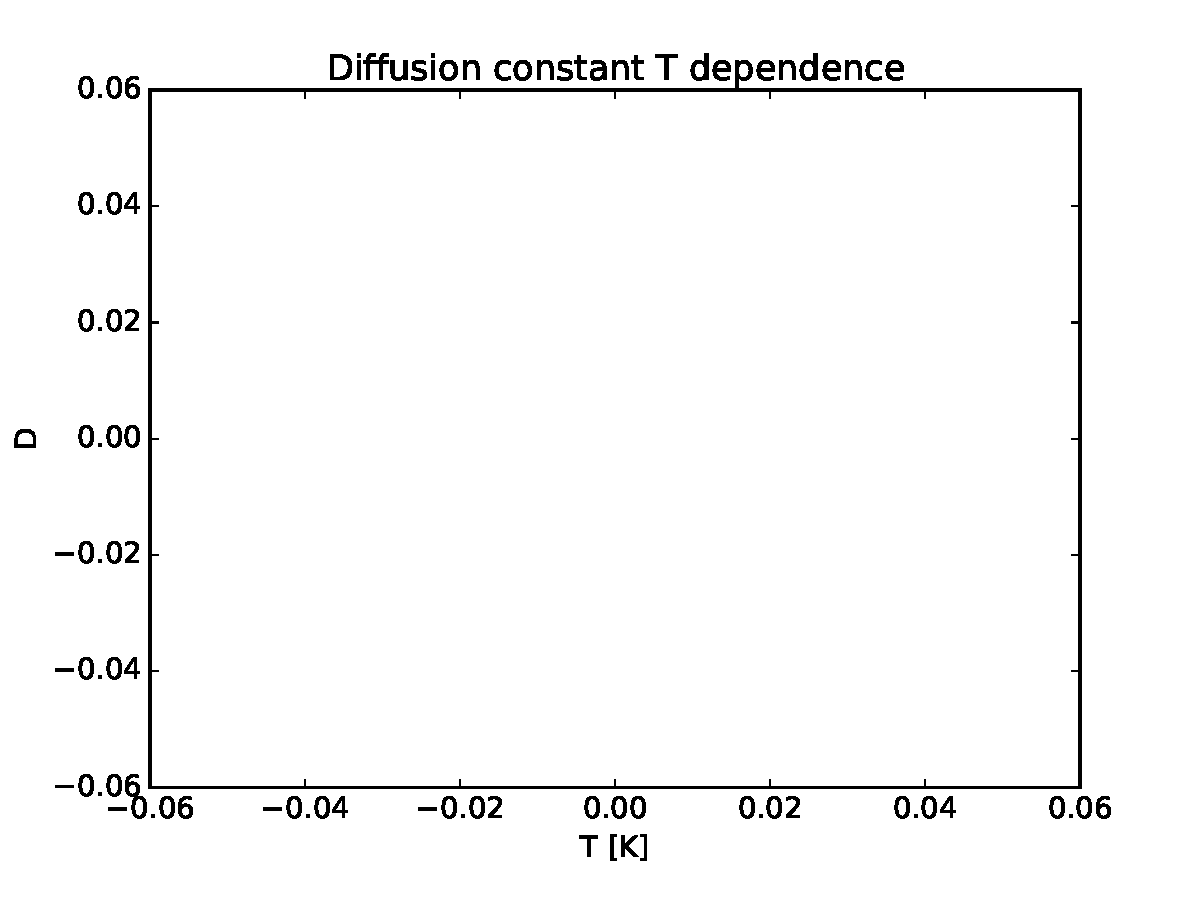
\includegraphics[width=0.8\linewidth]{../figures/diffusion_temp}\caption{This is a plot of the diffusion constant with respect to temperature. The values are taken from the slope of the linear regression of the mean squared distance versus time because of Einsteins relation (see Equation \ref.). The plos shows how the diffusion constant increases drastically after the melting point around 300 K.}\label{fig:diffusion_temp}
\end{figure}



------------------
Discuss benefits of periodic boundary conditions.

Why do the atoms have velocity from Maxwell-Boltzmann distribution?

What is the density?
